%#########################################################
\chapter{Diffusion Tensor Imaging}
\label{ch: Diffusion}
%#########################################################
Molecular diffusion in biological tissues is restricted due to interactions with many obstacles, such as fibers and neural tracts. 
Therefore diffusion patterns can be used to provide microscopic details about tissue architecture. This information is further used to detect abnormalities in skeletal muscles, heart and brain. 
MRI-based diffusion tensor imaging (DTI) is a relatively new modality, which allows the noninvasive \textit{in-vivo} determination of diffusion of water molecules arising from random motions due to the thermal energy of the tissue.
%-new paragraph-%

%-new paragraph-%
This chapter gives a brief introduction into diffusion theory and provides an overview of spin-echo and stimulated echo MR echo planar imaging pulse sequences that were used in the experiments discussed further in chapter~\ref{ch: DiffusionExp}.
%=========================================================
\section{Brownian Motion and Einstein Relation}
%=========================================================
In 1855 Adolf Fick explained diffusion through the flux of particles arising from the gradient of local concentration $c(\mathbf{r},t)$~\cite{Fick}:
%.........................................................
\begin{equation}\label{eq:Fick1}
\mathbf{J}=-D\nabla c(\mathbf{r},t)
\end{equation}
%.........................................................
For the total number of particles to be conserved divergence of the local flux should be related to the rate of change of $c(\mathbf{r},t)$ as $\nabla\mathbf{J}=-\frac{\partial c}{\partial t}$. This gives the diffusion equation:
%.........................................................
\begin{equation}\label{eq:Fick2}
\frac{\partial c}{\partial t}=D\nabla^2c
\end{equation}
%.........................................................
Equations~\ref{eq:Fick1} and \ref{eq:Fick2} are known as Fick's law. 
It was obtained for the case of admixture, when particles drift from higher to lower concentration regions, and this process is called \textit{mutual diffusion}. 
Albert Einstein in 1905 explained Brownian motion quantitatively~\cite{Einstein} and showed that Fick's laws are also valid for the case of \textit{self-diffusion}. 
Einstein described the motion of particles inside a finite volume $\delta V$ considering small displacements $\delta x$ due to the net force $K$, such that free energy is minimized: $\delta F=\delta E - T\delta S=0$. 
Utilizing the ideal gas model he related the work done by the particles with the change in entropy $\delta S = -k_B\frac{\partial V}{V}$. Thus the equilibrium condition is given:
%.........................................................
\begin{equation}\label{eq:EQ_Condition}
-Kn+k_BT\frac{\partial c}{\partial x}=0
\end{equation}
%.........................................................
where $k_B$ is Boltzmann's constant. The net flow of particles due to to net force $K$ is $J_{\mathrm{drift}}=\mu K $, where $\mu$ is mobility. Drift is counteracted by diffusive flow,  which according to Fick's law, is $J_{\mathrm{diff}}=-D\frac{\partial c}{\partial x}$. 
These flows are balanced and, together with equilibrium condition Equation~(\ref{eq:EQ_Condition}), result in a famous Einstein-Smoluchowski relation:
%.........................................................
\begin{equation}\label{eq:Einstein-Smoluchowski}
D=\mu k_BT
\end{equation}
%.........................................................
which was obtained independently by Albert Einstein~\cite{Einstein} in 1905, and Marian Smoluchowski~\cite{Smoluchowski} in 1906. 
For the small spherical particles of radius $r$, mobility is given by Stock's law $\mu=1/{(6\pi\eta r)}$, and Equation~(\ref{eq:EQ_Condition}) can be written in the following form:
%.........................................................
\begin{equation}\label{eq:Einstein-Stocks}
D=\frac{k_BT}{6\pi\eta r}
\end{equation}
%.........................................................
In addition to the expression for the diffusion coefficient, Einstein was able to describe  Brownian motion as a stochastic process~\cite{Einstein}. 
He considered conditional probability $P(\mathbf{r}|\mathbf{r'},t)$ for the particle at $\mathbf{r}$ at time $t_0=0$ to be at $\mathbf{r'}$ after time $t$. 
Local particle concentration~$c(\mathbf{r'}, t)$~is:
%.........................................................
\begin{equation}\label{eq:probability_concentration}
c(\mathbf{r'},t)=\int d\mathbf{r} \, c(\mathbf{r},0)P(\mathbf{r}|\mathbf{r'},t)
\end{equation}
%.........................................................
Since $c(\mathbf{r'},t)$ satisfies the diffusion equation Equation~(\ref{eq:Fick2}) for arbitrary choice of initial $c(\mathbf{r},0)$, the diffusion equation is also valid for probability $P(\mathbf{r'}|\mathbf{r}, t)$.
%.........................................................
\begin{equation}\label{eq:probability_diffusion}
\frac{\partial}{\partial t}P(\mathbf{r}|\mathbf{r'}t)=D\nabla^2P(\mathbf{r'}|\mathbf{r}, t)
\end{equation}
%.........................................................
With the initial condition $P(\mathbf{r'}|\mathbf{r}, 0)=\delta(\mathbf{r}-\mathbf{r'})$ the solution of the Equation~(\ref{eq:probability_diffusion}) is a Gaussian:
%.........................................................
\begin{equation}\label{eq:probability}
P(\mathbf{r}|\mathbf{r'},t)=\frac{1}{(4\pi Dt)^{3/2}} \mathrm{exp}\left( -\frac{(\mathbf{r'}-\mathbf{r})^2}{4Dt}\right)
\end{equation}
%.........................................................
From this equation, the mean square displacement is liner in time:
%.........................................................
\begin{equation}\label{eq:ms_dr}
\left<(\mathbf{r'}-\mathbf{r})^2\right>=6Dt
\end{equation}
%.........................................................
or in one dimension:
%.........................................................
\begin{equation}\label{eq:ms_dx}
\left<(x'-x)^2\right>=2Dt
\end{equation}
%.........................................................
The following definition of the diffusion coefficient flows from the Equation~(\ref{eq:ms_dx}):
%.........................................................
\begin{equation}\label{eq:D_v}
D=\lim_{t\rightarrow\infty}\frac{1}{2}\frac{\partial\left<\Delta x^2\right>}{\partial t}
\end{equation}
%.........................................................
Since $\Delta x = \int_0^t \mathrm{d}\tau \, v({\tau})$ the mean square displacement is:
%.........................................................
\begin{equation}\label{eq:D_v}
\left<\Delta x^2\right>=\int\limits_0^tdt_1\int\limits_0^tdt_2\left<v(t_1)v(t_2)\right>
\end{equation}
%.........................................................
By taking the derivative of this expression and using time translation invariance one can obtain Green-Kubo relation for diffusion coefficient $D$~\cite{Peliti}:
%.........................................................
\begin{equation}\label{eq:Green-Kubo}
D=\lim_{t \rightarrow \infty}\int\limits_0^\infty \mathrm{d} t \, \left<v(t) v(0)\right>
\end{equation}
%.........................................................
where $\left<v(t) v(0)\right>$ is the autocorrelation function of the molecular velocity $v$. In fact Equation~(\ref{eq:Green-Kubo}) represents a zero frequency component of the diffusion spectrum:
%.........................................................
\begin{equation}\label{eq:diffusion spectrum}
D(\omega)=\int\limits_0^\infty dt \, \left< v(t) v(0)\right> \mathrm{exp}(i\omega t) 
\end{equation}
%.........................................................
The correlation time is defined as:
%.........................................................
\begin{equation}\label{eq:correlation_time}
t_c=\int\limits_0^\infty dt \, \frac{\left<v(t) v(0)\right> }{\left< v^2\right>} 
\end{equation}
%.........................................................
and provides a timescale over which the fluctuating molecular velocity becomes decorrelated~\cite{DerekKJones}. 
This is an important result. 
In free solution, the correlation time is short. 
However, biological tissue molecules take much longer to thermalize because the length-scales of the spatial heterogeneities are typically much larger than the molecular scale. 
Thus in case of restricted diffusion, it's possible to access spectral features of the diffusion coefficient which provide detailed information even in case of complicated tissue architecture~\cite{Tuch:2002ts}.
%=========================================================
\section{Bloch-Torrey Equations and Diffusion Tensor}
%=========================================================
In 1950, just four years after the discovery of the NMR phenomenon by Bloch and Purcell~\cite{Bloch1946}, Ervin Hahn discovered that the spin-echoes he observed are sensitive to the effects of diffusion. 
He related the reduction of the signal to a dephasing caused by translational diffusion of spins subjected to local magnetic field gradients~\cite{Hahn}. 
In the presence of the diffusion term Bloch equations for the magnetization would change: 
%.........................................................
\begin{align}\label{eq:Bloch-Torrey}
\frac{dM_x}{dt}&=\gamma\left(\mathbf{M}\times B_0\right)_x-\frac{M_x}{\mathrm{T_2}}+D\Delta M_x\nonumber\\
\frac{dM_y}{dt}&=\gamma\left(\mathbf{M}\times B_0\right)_y-\frac{M_y}{\mathrm{T_2}}+D\Delta M_y\\
\frac{dM_z}{dt}&=\gamma\left(\mathbf{M}\times B_0\right)_z+\frac{M_0-M_z}{\mathrm{T_1}}+D\Delta(M_z-M_0)\nonumber
\end{align}
%.........................................................
This is so called Bloch-Torrey equations first introduced by Torrey in 1956~\cite{Torrey}.
Here $\mathbf{M}$ is the magnetization of a sample [\si{\ampere/\meter}], $B_0$ is a static magnetic field applied [\si{\tesla}], $\gamma$ is a gyromagnetic ratio [\si{\radian/\second \tesla}], $M_x$, $M_y$, $M_z$ are the $x$, $y$ and $z$ components of $\mathbf{M}, M_0$ is magnetization at thermal equilibrium and $\mathrm{T_1}, \mathrm{T_2}$ are the longitudinal and transversal relaxation times respectively. 
After \ang{90} radio frequency (RF) pulse is applied to the system, Bloch-Torrey equations give the following solution for the magnetization in the transverse plane:
%.........................................................
\begin{equation}\label{eq: dif_mag}
\bar{M}=M_0e^{-\frac{t}{T_2}}e^{-bD}
\end{equation}
%.........................................................
As opposed to the solution for the spin-echo Equation~(\ref{eq: dif_mag}) has an additional exponential factor $e^{-bD}$, \textit{b-}value identifies the measurement sensitivity to diffusion and determines the strength and duration of the diffusion gradients. The units of \textit{b-}value are [\si{\second/\milli\meter\squared}]:
%.........................................................
\begin{equation}\label{eq: b-value}
b=\gamma^2\int\limits_{0}^{\mathrm{TE}}dt\left(\int\limits_{0}^{t}dt'G(t')\right)^2
\end{equation}
%.........................................................
where $G$ is time-varying gradient of the magnetic field and $\mathrm{TE}$ is the echo-time.
Typical diffusion-weighted gradient consists of two lobes with equal area. In basic spin-echo sequences, two lobes ($G_{\mathrm{d1,2}}$) have the same polarity and are placed at either side of a refocusing RF-pulse as seen in Figure~\ref{fig: DTISeq}a. 
In gradient-echo sequences, however, the two lobes must have opposite polarity as shown in Figure~\ref{fig: DTISeq}b.
%*********************************************************
\begin{figure}[t]
\vspace{+0.2cm}
\centering
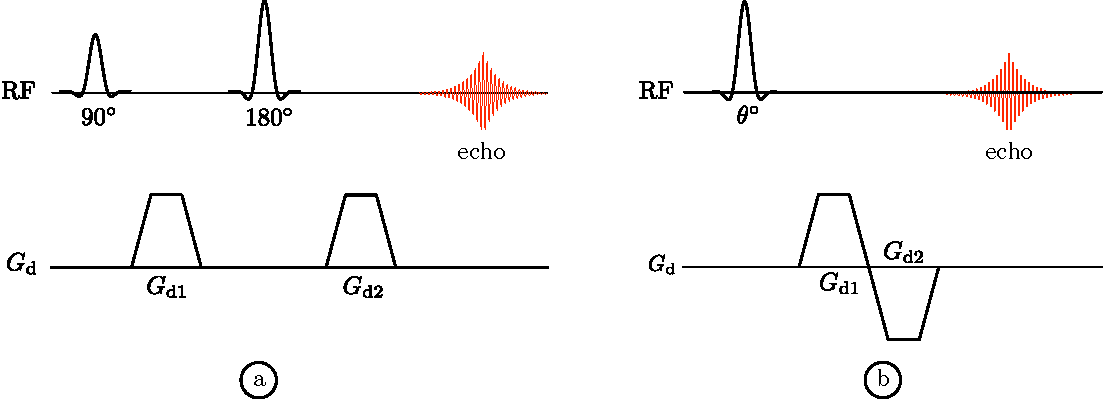
\includegraphics[width=\textwidth]{Figures/DiffusionPS.pdf}
\caption[Diffusion-weightning gradients in spin-echo and gradient echo pulse sequences]{Diffusion-weightning gradients in spin-echo and gradient echo pulse sequences.}\label{fig: DTISeq}
\end{figure}
%*********************************************************
An application of balanced bipolar gradients for the diffusion measurements was offered by Stejskal and Tanner~\cite{Stejskal}. 
Although the first gradient creates a spatially dependent phase to each spin the second gradient eliminates this effect for the stationary spins. 
Each of the protons experiencing a random diffusive displacement between the application of the two gradient pulses will acquire a phase offset proportional to the magnitude of the displacements. 
The result is phase dispersion proportional to the spread of positions. Thus, the diffusion coefficient $D$ along any direction can be measured by comparing MR signals $S(b)=M_0e^{-t/\mathrm{T_2}}e^{-bD}$ and $S(0)=M_0e^{-t/\mathrm{T_2}}$:
\begin{equation}\label{eq: Diffusion from bvalue}
D=-\frac{1}{b}\ln{\frac{S(b)}{S(0)}}
\end{equation}
%.........................................................
Until now diffusion coefficient $D$ was considered as a scalar in anisotropic medium. 
Biological tissues with regularly ordered microstructure such as skeletal muscle, spine, tongue, heart, white matter exhibit anisotropic water diffusion. 
An anisotropic media can be described in terms of tensor formalism. 
A diffusion tensor is a covariant tensor of $\rank$~2 that is described by a $3\times3$ symmetric matrix with 6 unique elements:
%.........................................................
\begin{equation}
\mathbf{D} =\left[
\begin{array}{ccc}
D_{xx} & D_{xy} & D_{xz} \\[4pt]
D_{yx} & D_{yy} & D_{yz} \\[4pt]
D_{zx} & D_{zy} & D_{zz} \\
\end{array}\right]
\end{equation}
%.........................................................
The components of the diffusion tensor can be calculated from the diffusion weighted image (DWI) set collected with the diffusion gradients applied in six or more directions. 
For the arbitrary number of gradient directions $n \geq 6$, the following system of liner equations can be written:
%.........................................................
\begin{align}
\begin{cases}
-\ln{\dfrac{S(b_1)}{S(b_0)}}&=\displaystyle\sum_{i,j=1}^3 b_{1ij}D_{ij}\\[2em]
-\ln{\dfrac{S(b_2)}{S(b_0)}}&=\displaystyle\sum_{i,j=1}^3 b_{2ij}D_{ij}\\
&\setbox0\hbox{=}\mathrel{\makebox[\wd0]{\vdots}} \\
-\ln{\dfrac{S(b_n)}{S(b_0)}}&=\displaystyle\sum_{i,j=1}^3 b_{nij}D_{ij}\\
\end{cases}
\end{align}
%.........................................................
where indexes $i$ and $j$ stand for $x,y$ and $z$ components.
Diffusion tensor yields several useful metrics. Mean Apparent Diffusion Coefficient (ADC) which gives the magnitude of the diffusion:
%.........................................................
\begin{equation}
\mathrm{ADC}=\frac{1}{3}\mathrm{Tr}\mathbf{D}
\end{equation}
%.........................................................
And  fractional anisotropy (FA) which is calculated after diffusion tensor eigenvalue decomposition is performed:
%.........................................................
\begin{equation}
\mathrm{FA}=\frac{\sqrt{3\displaystyle\sum_{i=1}^3 (\lambda_i-\mathrm{ADC})^2}}{\sqrt{2\displaystyle\sum_{i=1}^3 \lambda_i^2}}
\end{equation}
%.........................................................
where $\lambda_{1,2,3}$ are the eigenvalues of the diffusion tensor.
FA describes the degree of anisotropy and can take values between zero and one. 
Conventionally diffusion tensors are represented by ellipsoids.
%*********************************************************
\begin{figure}[h]
\vspace{+0.2cm}
\centering
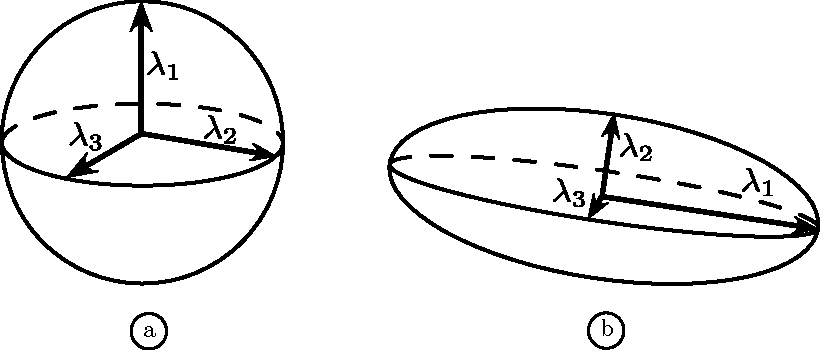
\includegraphics[scale=0.8]{Figures/DiffusionFA.pdf}
\caption[Visual representation of the diffusion tensor in the isotropic and anisotropic cases]{Visual representation of the diffusion tensor in the isotropic and anisotropic cases.}\label{fig: AnisIso}
\end{figure}
%*********************************************************
\noindent If $\mathrm{FA} = 1$, then diffusion occurs only along one axis and is fully restricted along all others. $\mathrm{FA} = 0$ means an isotropic diffusion (Figure~\ref{fig: AnisIso}a). 
Biological tissues, such as muscle are anisotropic (Figure~\ref{fig: AnisIso}b) and diffusion mostly occurs along one of the eigenvectors, being restricted along the remaining two.
%=========================================================
\section{Echo Planar Imaging (EPI)}
\label{sec: EPI}
%=========================================================
A conventional MRI spin echo sequence acquires \textit{k}-space by sequential repetition of the basic spin echo pulse sequence ($\SI{90}{\degree}$ excitation RF-pulse followed by refocusing $\SI{180}{\degree}$). 
This sequence is too long compared to physiological (patient) motion. 
Addition of diffusion sensitization to routine spin echo sequence will essentially result in a completely wiped out image. 
In order to freeze motion, the established method for performing diffusion weighted imaging is to use a single shot technique, a spin echo echo-planar imaging (EPI) sequence, rather than a conventional spin echo.
%-new paragraph-%

%-new paragraph-%
Echo planar imaging (EPI) is the fastest MRI pulse sequence. 
With the modern hardware EPI allows producing of a 2D image as fast as tens of a millisecond. 
The main difference of EPI pulse sequence from the conventional pulse sequences (such as spin echo and gradient echo), is that the entire \textit{k}-space is acquired with one RF excitation (single-shot)~\cite{RNDT23}. 
This is accomplished by a series of bipolar readout gradients. 
To generate a train of gradient echoes (Figure~\ref{fig: EPI}a) with accompanying small phase-encoding gradients ('blips'), each gradient echo is distinctively spatially encoded so that multiple \textit{k}-space lines can be sampled under an RF spin echo (Figure~\ref{fig: EPI}b).
%*********************************************************
\begin{figure}[!h]
\vspace{+0.2cm}
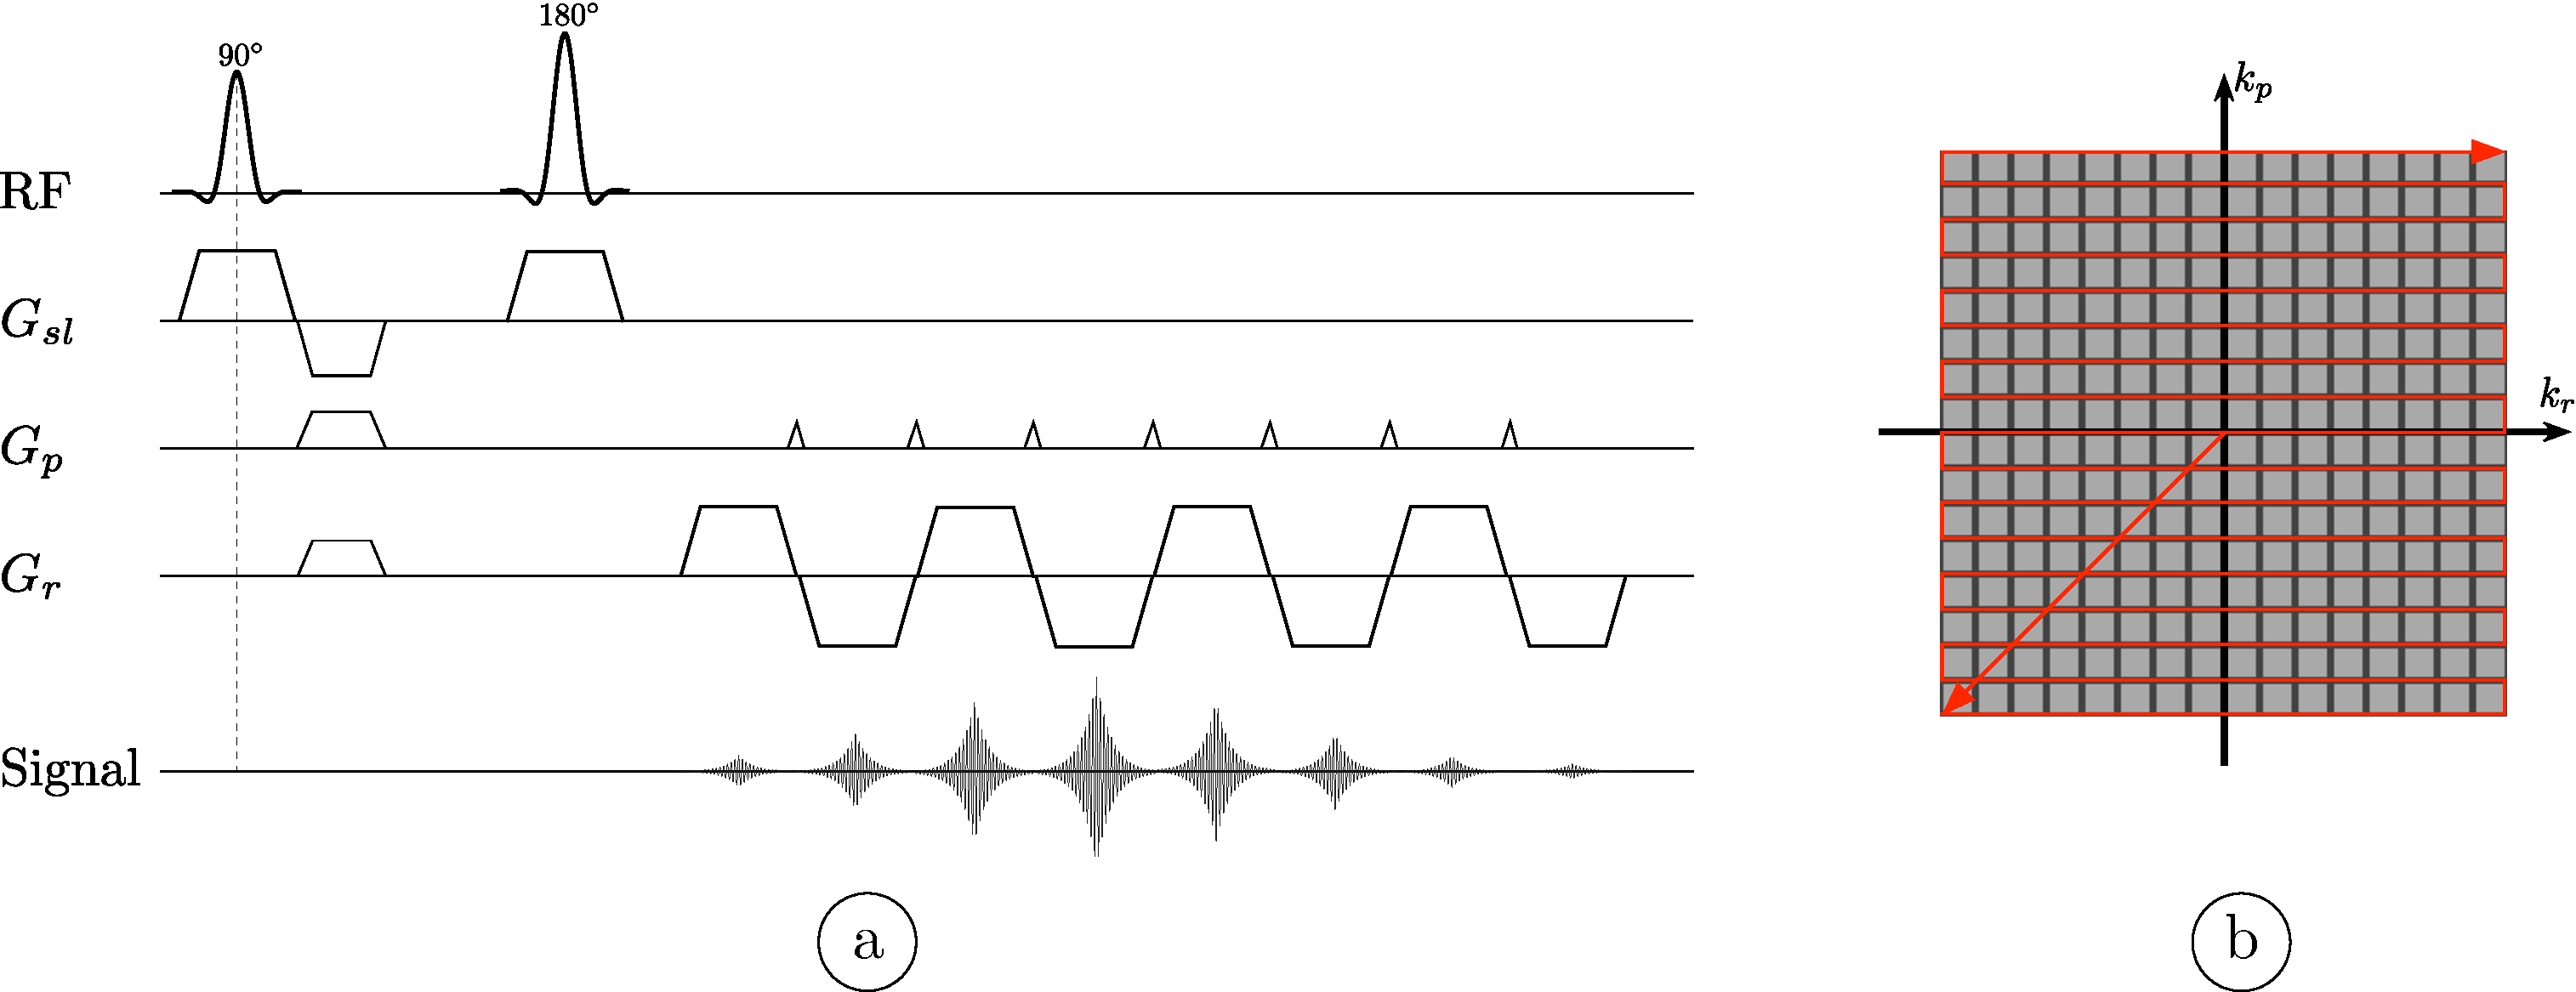
\includegraphics[width=\textwidth]{Figures/EPI.pdf}
\caption[Spin-echo diffusion weighted EPI sequence and \textit{k}-space sampling path]{Spin-echo diffusion weighted EPI sequence and \textit{k}-space sampling path.}\label{fig: EPI} 
\end{figure}
%*********************************************************
EPI generates an image in a considerably shorter time than any other MRI sequence. 
Typical EPI pulse sequence is capable of producing $\sim 100$ gradient echoes as a result 2D image can be constructed from a single RF excitation~\cite{RNDT24}.
%-new paragraph-%

%-new paragraph-%
Compared to conventional MR imaging pulse sequences, EPI is more prone to a variety of artifacts. 
These artifacts arise from the fact the effective bandwidth in the phase-encoding direction is very small so that small differences in the frequency (other than from the phase encode gradient) at different spatial locations can result in severe mismapping. 
These frequency differences occur due to eddy currents from the large diffusion gradients, as well as from magnetic field inhomogeneities arising primarily from susceptibility differences in tissues and air. 
In my studies several correction techniques for eddy current, strong steady field inhomogeneity magnetic susceptibility were incorporated at the image pre-processing stage.
%-new paragraph-%

%-new paragraph-%
In spin-echo EPI sequence diffusion gradients are applied right before and immediately after $\SI{180}{\degree}$ refocusing pulse. 
As a result the range of the diffusion times is very constrained. 
Ability to measure diffusion tensor at diffusion times much longer compared to spin-echo EPI sequence provides an extra dimension in the data and a better estimate for micro-structural parameters.
%~~~~~~~~~~~~~~~~~~~~~~~~~~~~~~~~~~~~~~~~~~~~~~~~~~~~~~~~~
\subsection{Stimulated Echo Acquisition Mode (STEAM)}
%~~~~~~~~~~~~~~~~~~~~~~~~~~~~~~~~~~~~~~~~~~~~~~~~~~~~~~~~~
Compared to spin-echo which uses two RF-pulses Stimulated Echo~\cite{Hahn} uses three $\SI{90}{\degree}$ pulses with the same phase and observes total of five echos: three primary spin echos, one secondary and one simulated echo. 
All primary and a secondary echo experience $\mathrm{T_2^*}$ dephasing in between second and third RF-pulses while the magnetization forming stimulated echo is preserved along the longitudinal axis. 
The phase evolution of the magnetization in the pulse sequence with three RF-pulses is conveniently described using the diagram from~Figure~\ref{fig: STEAM_phase}.
%*********************************************************
\begin{figure}[!h]
\vspace{+0.2cm}
\centering
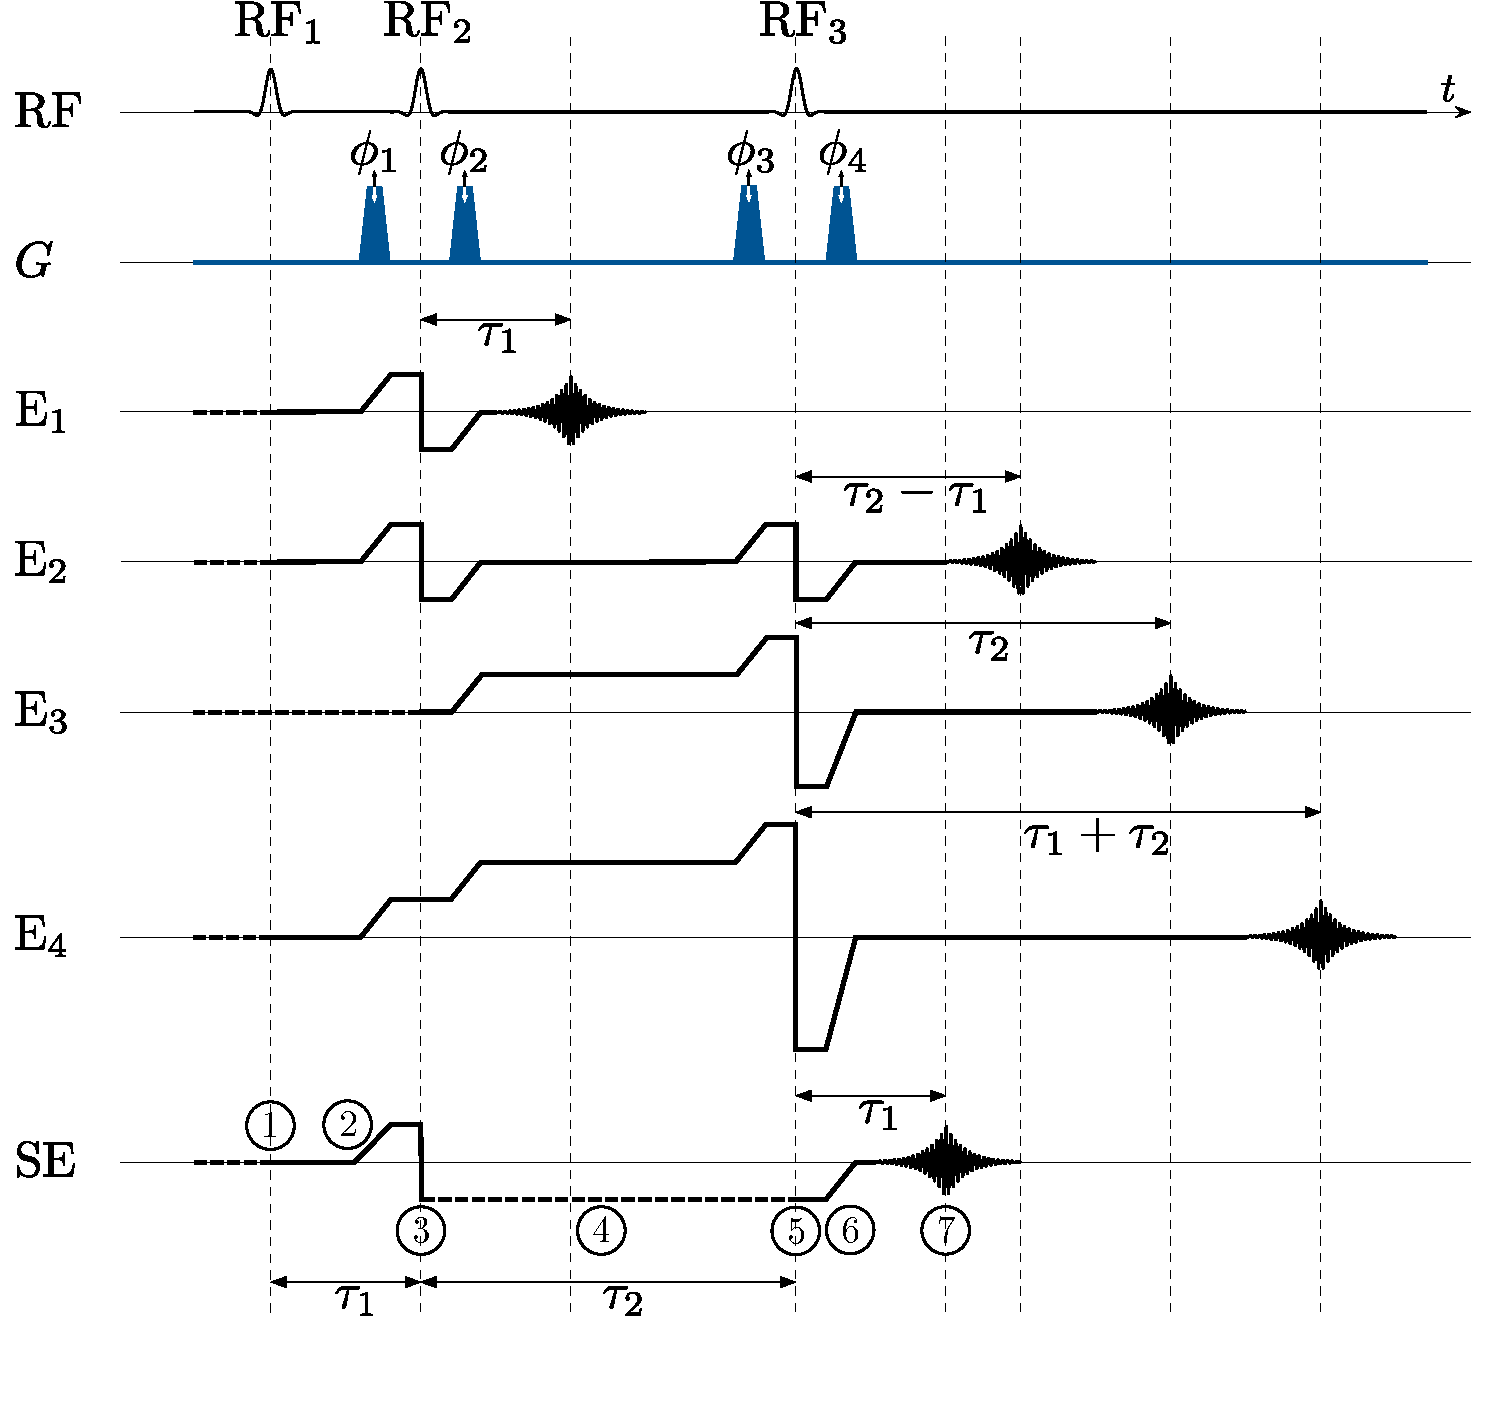
\includegraphics[width=\textwidth]{Figures/STEAM_Phase.pdf}
\caption[Spin phase evolution diagram for the pulse sequence with three RF-pulses]{Spin phase evolution diagram for the pulse sequence with three RF-pulses.}\label{fig: STEAM_phase} 
\end{figure}
%*********************************************************
 To keep only simulated echo pathway while eliminating signal from all the other four echoes as well as signal from free induction decays a set of four crusher gradients $\phi_{1-4}$ must be introduced. 
 For signal to be produced the accumulated phase due to the crusher must cancel out. 
 Phase dispersion created by a crusher gradient is directly proportional to its area thus by manipulating the size of the crusher gradients $\phi_{1-4}$ the stimulated echo pathway can be chosen while other echos can be destroyed.
%-new paragraph-%

%-new paragraph-%
 The stimulated echo signal pathway denoted SE in~Figure~\ref{fig: STEAM_phase}: first $\mathrm{RF_1}$ excites magnetization (1), next, phase is accumulated (2) due to gradient $\phi_1$, then $\mathrm{RF_2}$ reverses the phase (3) and locks magnetization longitudinally (4), following $\mathrm{RF_3}$ magnetization is restored in the transverse plane(5) and rephased by crusher gradient $\phi_4$ (6) to form an echo (7).
%-new paragraph-%

%-new paragraph-%
Conditions for stimulated echo are the following:
%.........................................................
\begin{equation}\label{eq: STEAM phase}
{\setstretch{1.0}
\begin{cases}
    \mathrm{E_1} &= -\phi_1 + \phi_2\\
    \mathrm{E_2} &= -\phi_1 + \phi_2 + \phi_3 - \phi_4\\
    \mathrm{E_3} &= -\phi_2 + \phi_3 + \phi_4\\
    \mathrm{E_4} &= -\phi_1 - \phi_2 - \phi_3 + \phi_4\\
    \mathrm{E_{1-4}} &\neq 0\\
    \mathrm{SE} &= -\phi_1 + \phi_4\\
    \phi_2 &\neq 0\\
    \phi_4 &\neq 0\\
\end{cases}
}
\end{equation}
%.........................................................
where first five equations are the conditions to destroy four echos, last two equations are conditions to remove signal originating from free induction decay and the equation for SE is the requirement to preserve stimulated echo. 
Diffusion weighting is added into the STEAM sequence by placing two identical diffusion gradients: first is placed in between $\mathrm{RF_1}$ and $\mathrm{RF_2}$ and second after $\mathrm{RF_3}$ pulse.
%~~~~~~~~~~~~~~~~~~~~~~~~~~~~~~~~~~~~~~~~~~~~~~~~~~~~~~~~~
\subsection{Correction to the \textit{b}-matrix}
\label{subsection: STEAM b value}
%~~~~~~~~~~~~~~~~~~~~~~~~~~~~~~~~~~~~~~~~~~~~~~~~~~~~~~~~~
In STEAM diffusion weighted sequence contribution to the \textit{b-}matrix (Equation~\ref{eq: bmatrix}) from cross-terms between different gradients becomes significant at long diffusion time $\Delta$ and must be calculated from the Equation~\ref{eq: b-value}. 
%.........................................................
\begin{equation}\label{eq: bmatrix}
b =\left[
\begin{array}{ccc}
b_{rr} & b_{rp} & b_{rs} \\
b_{pr} & b_{pp} & b_{ps} \\[1pt]
b_{sr} & b_{sp} & b_{ss} \\
\end{array}\right]
\end{equation}
%.........................................................
where indices $r, p, s$ are corresponding to three gradient axis: readout, phase encoding and slice selection respectively. 
%-new paragraph-%

%-new paragraph-%
Figure~\ref{fig: STEAM_GE} shows a plot of STEAM pulse sequence programmed in EPIC (GE Medical Systems, Milwaukee, WI, USA). 
Important timing parameters marked: diffusion time ($\Delta$) measured as time between diffusion gradients, duration of the diffusion gradients ($\delta$) and mixing time TM, measured as time between centers of the second and third RF-pulses.
%*********************************************************
\begin{figure}[h]
\vspace{+0.2cm}
\centering
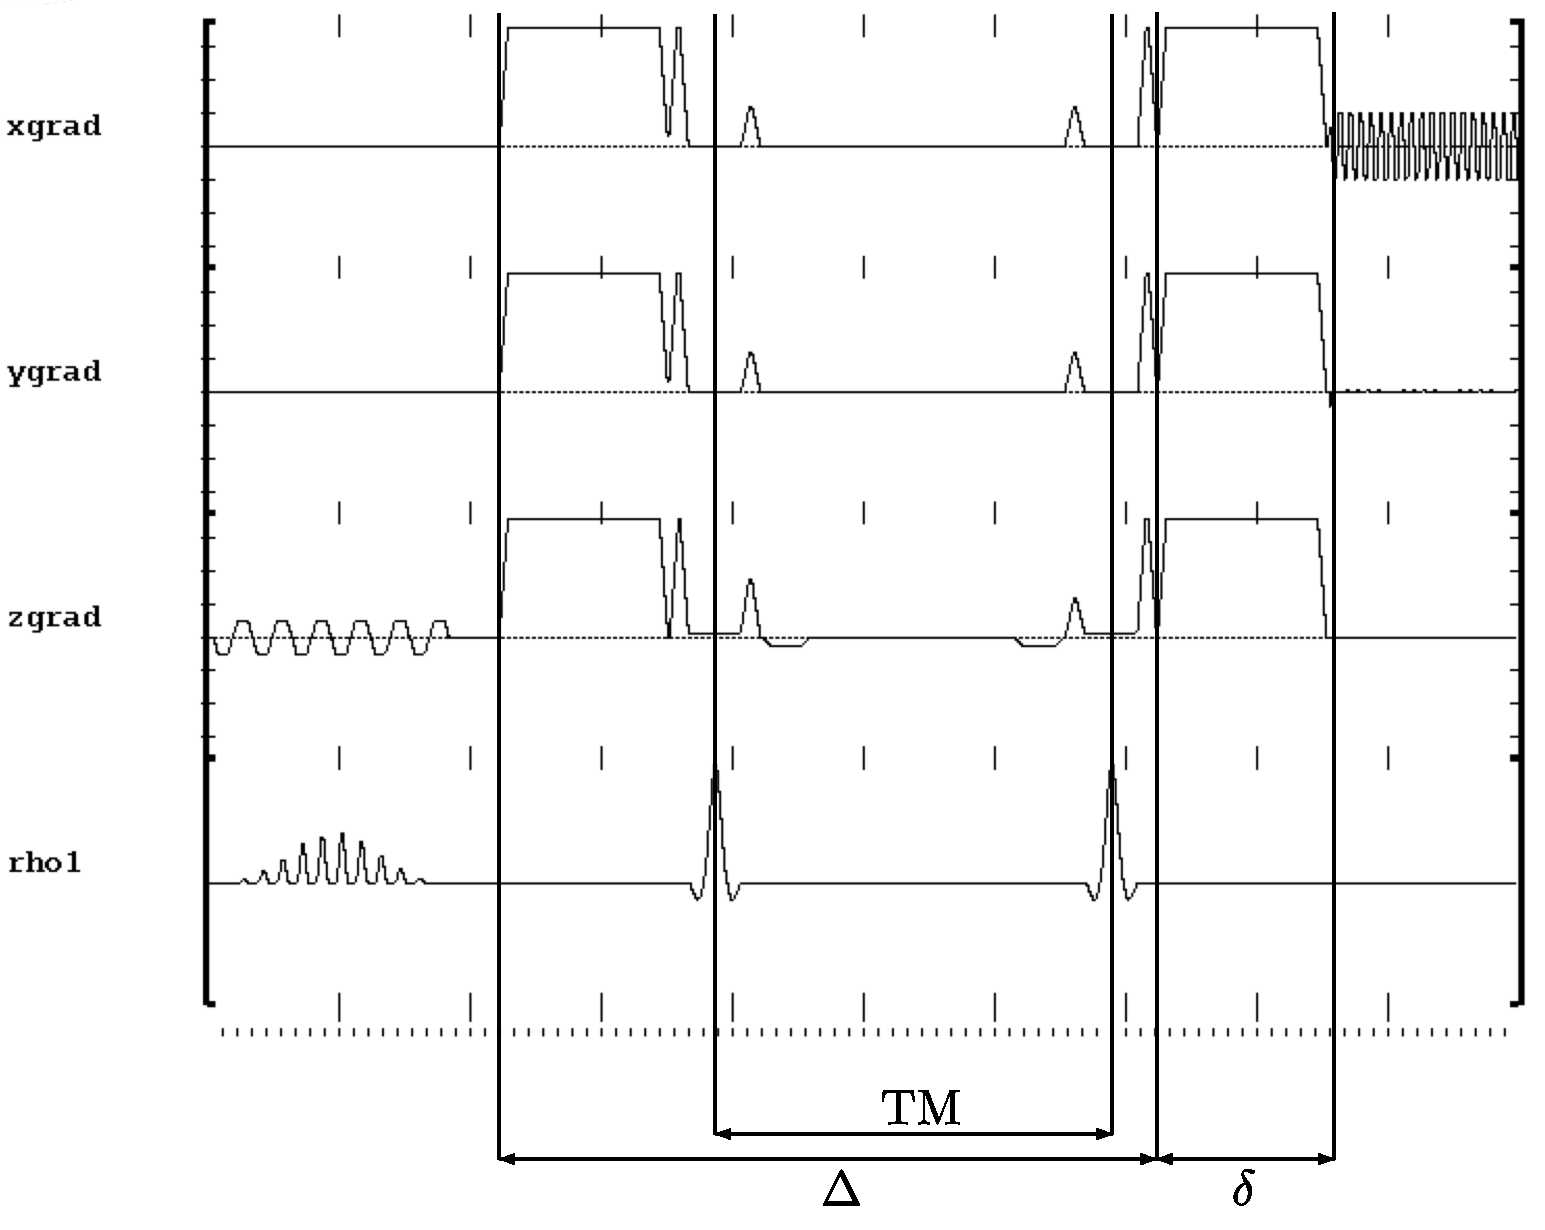
\includegraphics[width =0.7\textwidth]{Figures/STEAM_GE.pdf}
\caption[Plot of STEAM pulse sequence programmed for GE scanner]{Plot of STEAM pulse sequence programmed for GE scanner.}\label{fig: STEAM_GE} 
\end{figure}
%*********************************************************
To satisfy conditions~\ref{eq: STEAM phase} the following configuration of crusher gradients was chosen:
%.........................................................
\begin{equation}\label{eq: bmatrix}
{\setstretch{1.0}
\begin{cases}
    \phi_1 = \phi_4\\
    \phi_1 \neq \phi_2\\
    \phi_2 \neq 0\\
    \phi_4 \neq 0\\
    \phi_2 \neq - \phi_3\\
    \phi_3 \neq \phi_2 - \phi_1\\
    \phi_3 \neq 2\phi_1 - \phi_2\\
    \phi_3 < \phi_2 < \phi_1
\end{cases}
}
\end{equation}
%.........................................................
Using full analytic form derived in~\cite{RNDT} independent components for \textit{b-}matrix due to diffusion, crusher and slice select gradient interactions are:
%.........................................................
\begin{equation}\label{eq: bmatrix}
{\setstretch{1.0}
\begin{array}{l}
    b_{rr} = \gamma^2\Bigl[G_{\mathrm{d}r}^2\tau_{11} + 2G_{\mathrm{d}r}G_{\mathrm{c}r}\tau_{12} + G_{\mathrm{c}r}^2\tau_{22}\Bigr]\\[10pt]
    
    b_{pp} = \gamma^2\Bigl[G_{\mathrm{d}p}^2\tau_{11} + 2G_{\mathrm{d}p}G_{\mathrm{c}p}\tau_{12} + G_{\mathrm{c}p}^2\tau_{22} \Bigr]\\[10pt]
    
    b_{ss} = \gamma^2\Bigl[G_{\mathrm{d}s}^2\tau_{11} +2G_{\mathrm{d}s}G_{\mathrm{c}s}\tau_{12} + G_{\mathrm{c}s}^3\tau_{22} + G_{\mathrm{sl}}^2\tau_{33} \Bigr]\\[10pt]
    
    b_{rp} = b_{pr} = \gamma^2\Bigl[G_{\mathrm{d}r}G_{\mathrm{d}p}\tau_{11} + \left(G_{\mathrm{c}p}G_{\mathrm{d}r} + G_{\mathrm{c}r}G_{\mathrm{d}p}\right)\tau_{12} + G_{\mathrm{c}r}G_{\mathrm{c}p}\tau_{22} \Bigr]\\[10pt]
    
    \begin{split}
	b_{rs} &= b_{sr} = \gamma^2\Bigl[G_{\mathrm{d}s}G_{\mathrm{d}r} \tau_{11} + \left( G_{\mathrm{d}s}G_{\mathrm{c}r} + G_{\mathrm{d}r}G_{\mathrm{c}s}\right)\tau_{12} + \\[2pt]
    	 	&\qquad\qquad\qquad\quad  + G_{\mathrm{c}r}G_{\mathrm{c}s}\tau_{22} + G_{\mathrm{sl}}G_{\mathrm{d}r}\tau_{13}+G_{\mathrm{sl}}G_{\mathrm{c}r}\tau_{23}\Bigr]
	\end{split}
    \\[4ex]
    \begin{split}
	b_{ps} &= b_{sp} = \gamma^2 \Bigl[G_{\mathrm{d}s}G_{\mathrm{d}p} \tau_{11} + \left( G_{\mathrm{d}s}G_{\mathrm{c}p} + G_{\mathrm{d}p}G_{\mathrm{c}s}\right)\tau_{12} + \\[2pt]
    	 	&\qquad\qquad\qquad\quad  + G_{\mathrm{c}p}G_{\mathrm{c}s}\tau_{22} + G_{\mathrm{sl}}G_{\mathrm{d}p}\tau_{13}+G_{\mathrm{sl}}G_{\mathrm{c}p}\tau_{23}\Bigr]\\[4pt]
	\end{split}
    \end{array}
}
\end{equation}
%.........................................................
with gradients amplitudes: $G_{\mathrm{d}*}$ and $G_{\mathrm{c}*}$ being diffusion and crusher pulses respectively where $*$ denotes gradient axis ($r,p$ or $s$), $G_{\mathrm{sl}}$ being an amplitude of a slice selection gradient pulse. 
Time constants $\tau_{ij}$ for the trapezoid gradient shape approximation are:
%.........................................................
\begin{equation}\label{eq: bmatrix timing}
{\setstretch{1.0}
\begin{array}{l}
	
	\tau_{11} = \delta_1^2\left( \Delta_1 - \dfrac{1}{3}\delta_1\right) + \dfrac{1}{30}\epsilon_{\mathrm{d}}^3-\dfrac{1}{6}\delta_1\epsilon_{{\mathrm{d}}}^2\\[12pt]
	\tau_{22} = \delta_2^2\left( \Delta_2 - \dfrac{1}{3}\delta_2\right) + \dfrac{1}{30}\epsilon_{\mathrm{c}}^3-\dfrac{1}{6}\delta_2\epsilon_{{\mathrm{c}}}^2\\[12pt]
	\tau_{12} = \delta_1\delta_2\Delta_2\\[12pt]
	\tau_{13} = \dfrac{1}{4}\delta_1\delta_{\mathrm{sl}}^2\\[12pt]
	\tau_{23} = \dfrac{1}{4}\delta_2\delta_{\mathrm{sl}}^2\\[12pt]
	\tau_{33} = \dfrac{1}{12}\delta_{\mathrm{sl}}^3\\[12pt]
\end{array}
}
\end{equation}
%.........................................................
where $\Delta_1$ is diffusion time, time constant $\Delta_2$ and pulse durations $\delta_{1,2}$ defined:
%.........................................................
\begin{equation}\label{eq: bmatrix timing delta}
{\setstretch{1.0}
\begin{array}{l}
	\Delta_{2} = \Delta_{1}-(\delta_{\mathrm{d}}+\delta_{\mathrm{c}})-2(\epsilon_{\mathrm{d}}+\epsilon_{\mathrm{c}})\\[12pt]
	\delta_{1} = \delta_{\mathrm{d}}+\epsilon_{\mathrm{d}}\\[12pt]
	\delta_{2} = \delta_{\mathrm{c}}+\epsilon_{\mathrm{c}}
\end{array}
}
\end{equation}
%.........................................................
$\delta_{\mathrm{d}}$ and $\delta_{\mathrm{c}}$ durations of the diffusion and crusher gradients, $\epsilon_{\mathrm{d}}$ and $\epsilon_{\mathrm{c}}$ rise time of the diffusion and crusher gradients, $\delta_{\mathrm{sl}}$ duration of the slice selection gradient.
	
	